\section{Simulation Analysis}
\label{sec:simulation}

\paragraph{} Given the input signal of the circuit is sinusoidal the voltage and current values vary with time, and it is relevant to know how the two parameters evovlve with time. 
We also ran an operating point analysis to confirm the forward-active region operation of the two transients. We also ran a frequency response analysis, in order to see the gain and
 bandwith of the amplified signal.

\subsection{Operating Point Analysis}

\paragraph{} In the table bellow we can see the resuls obtained from the operating point analysis.

\begin{table}[h]
  \centering
  \begin{tabular}{|l|r|}
    \hline    
    {\bf Name} & {\bf Values [V]} \\ \hline
    v(1) & 0.000000e+00\\ \hline
v(2) & 1.662312e-15\\ \hline
v(3) & 5.127494e-15\\ \hline
v(5) & 1.417269e-15\\ \hline
v(6) & 8.511786e+00\\ \hline
v(7) & -8.18711e-16\\ \hline
v(8) & -1.77636e-15\\ \hline
v(9) & -8.18711e-16\\ \hline
 
  \end{tabular}
  \caption{Operating point node voltage values of the amplifier circuit.}
  \label{tab:operator}
\end{table}

\paragraph{} The voltages in nodes in and in2 are zero, which is expected given that the source as no DC component. Likewise, the the voltage in node out is zero, since the output 
coupling capacitor blocks the incoming DC voltage.

\paragraph{} We can also see that Vcoll > Vbase > Vemit, which is antecipated due to the operation of the npn transistor. Vemit2 > Vcoll > GND, which is also expected, sinse the pnp 
transistor operation ensures that the voltage drop occurs from the emitter to the collector. Therefore, both our transistors work in the PFA.

\subsection{Frequancy Response and Impedances}

\paragraph{} We measured the input impedance, seen from the source point of view, and the output impedance, see from the output pointe of view.

\begin{figure}[!h] \centering
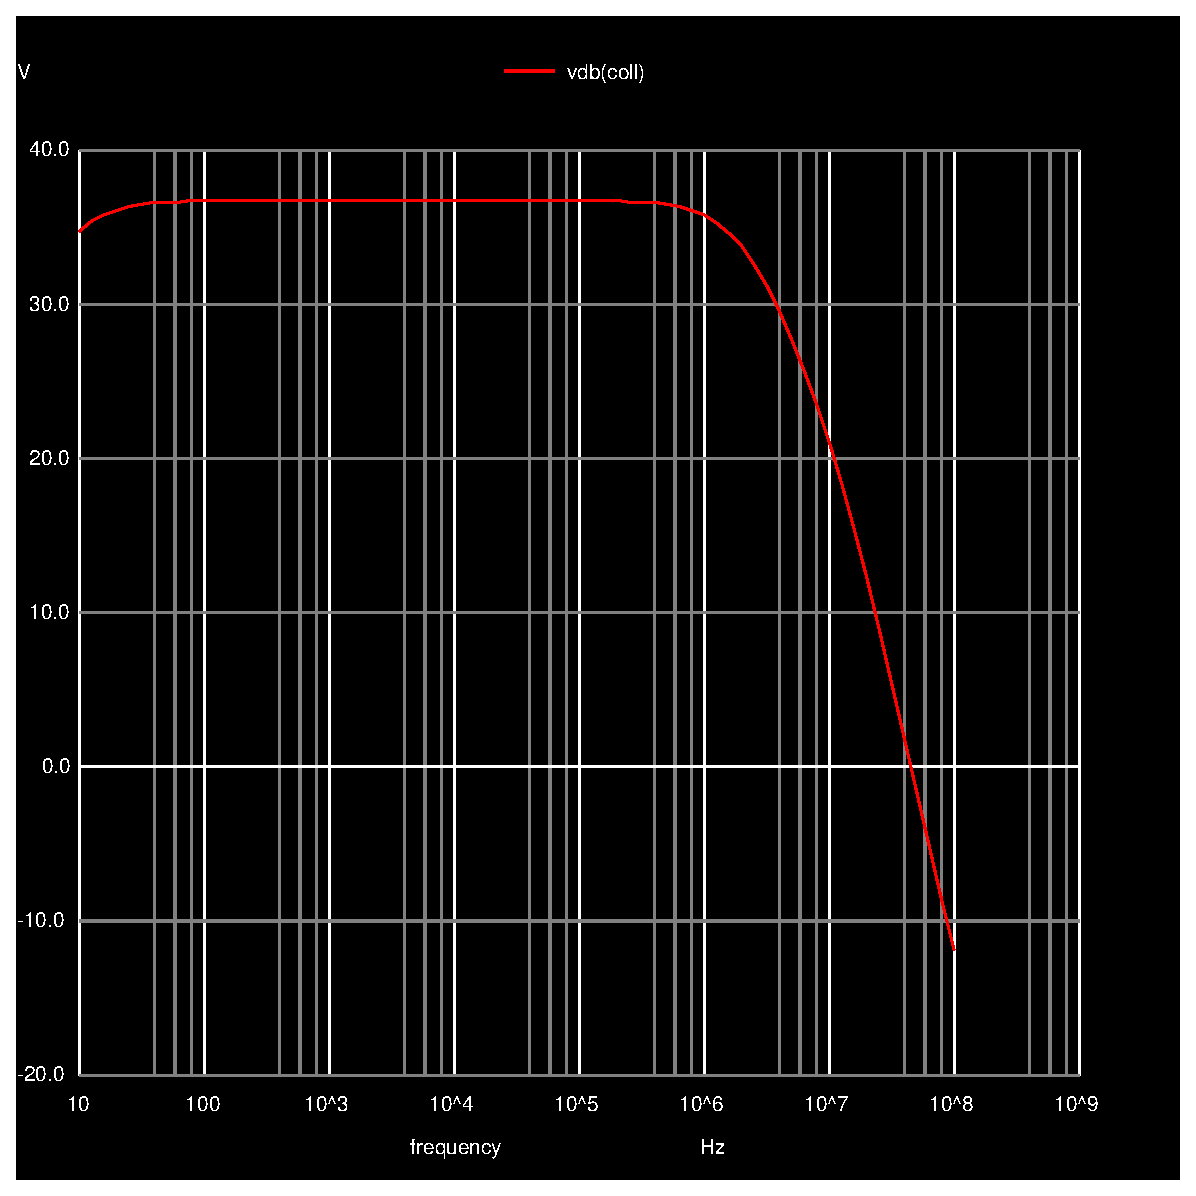
\includegraphics[width=0.6\linewidth]{stage.eps}
\caption{Gain Stage output voltage gain (frequency response).}
\label{fig:gainstage}
\end{figure}

\begin{figure}[!h] \centering
\includegraphics[width=0.6\linewidth]{output.eps}
\caption{Load output voltage gain (frequency response).}
\label{fig:outputstage}
\end{figure}

\paragraph{} As we can see in the graphs above, the gain graph has traits of a band-pass filter, filtering frequencies that are not medium.

\begin{table}[h]
  \centering
  \begin{tabular}{|l|r|}
    \hline    
    {\bf Name} & {\bf Values} \\ \hline
    Gain  & 72.4597\\ \hline
Gain(dB) & 37.2019\\ \hline
Lower cut-off frequency & 19.9876 Hz\\ \hline
Upper cut-off frequency & 2.32455E+06 Hz\\ \hline
Bandwidth & 2.32453E+06 Hz\\ \hline
Input impedance & 0.633365 kOhm\\ \hline

    Output impedance & 0.681719 + j*-0.46675 kOhm\\ \hline
Output impedance modulus & 0.826194 kOhm\\ \hline
Output impedance phase & -34.3981 degrees\\ \hline
     
  \end{tabular}
  \caption{Output gain, bandwidth, and input and output impedances of the audio amplifier circuit (as a whole).}
  \label{tab:main}
\end{table}

\paragraph{} In the table above we can see the results obtained.

\paragraph{} Finally, graph bellow compares the input and output signals, and we can conclude that the objective of the lab as achieved, this is, amplify the input signal. I this case, the imput signal 
was amplified 50 times.

\begin{figure}[!h] \centering
\includegraphics[width=0.6\linewidth]{comp.eps}
\caption{Evolution of the AC signal from input to output.}
\label{fig:comp}
\end{figure}

\begin{table}[h]
  \centering
  \begin{tabular}{|l|r|}
    \hline    
    {\bf Name} & {\bf Values} \\ \hline
    1/ (515.8* ((maximum(v(5))-minimum(v(5))) + abs(mean(v(5)-12)) + 10e-6)) & 7.528792e-04\\ \hline
 
  \end{tabular}
  \caption{Cost and merit of the audio amplifier circuit.}
  \label{tab:merit}
\end{table}

\clearpage
